\documentclass{article}
\usepackage{bm}
\usepackage{amsmath}
\usepackage{graphicx}
\usepackage{mdwlist}
\usepackage[colorlinks=true]{hyperref}
\usepackage{geometry}
\usepackage{kotex}
\geometry{margin=1in}
\geometry{headheight=2in}
\geometry{top=2in}
\usepackage{palatino}
%\renewcommand{\rmdefault}{palatino}
\usepackage{fancyhdr}
\usepackage{indentfirst}

\newcommand{\red}[1]{{\color{red} #1}}
\newcommand{\blue}[1]{{\color{blue} #1}}
\newcommand{\orange}[1]{{\color{orange} #1}}
\newcommand{\purple}[1]{{\color{purple} #1}}

%\pagestyle{fancy}
\rhead{}
\lhead{}
\chead{%
  {\vbox{%
      \vspace{2mm}
      \large
      Statistics Lab 033.020\hfill
\\
      Seoul National University
      \\[4mm]
      \textbf{Assignment \#3} \\
      \texttt{2016-19516, Sangjun Son}
    }
  }
}

%%%%%%%%%%%%%%%%%%%%%%%
\usepackage{xcolor}
\usepackage{listings}
\definecolor{vgreen}{RGB}{104,180,104}
\definecolor{vblue}{RGB}{49,49,255}
\definecolor{vorange}{RGB}{255,143,102}

\lstdefinestyle{r-style}
{
    language=R,
    basicstyle=\footnotesize\ttfamily,
    keywordstyle=\color{vblue},
    identifierstyle=\color{black},
    commentstyle=\color{vgreen},
    numbers=left,
    numberstyle=\tiny\color{black},
    numbersep=10pt,
    tabsize=8,
    moredelim=*[s][\colorIndex]{[}{]},
    literate=*{:}{:}1
}

\lstdefinestyle{out-style}
{
    language=R,
    basicstyle=\footnotesize\ttfamily,
    numbersep=10pt,
    tabsize=8,
    moredelim=*[s][\colorIndex]{[}{]},
    literate=*{:}{:}1
}

\makeatletter
\newcommand*\@lbracket{[}
\newcommand*\@rbracket{]}
\newcommand*\@colon{:}
\newcommand*\colorIndex{%
    \edef\@temp{\the\lst@token}%
    \ifx\@temp\@lbracket \color{black}%
    \else\ifx\@temp\@rbracket \color{black}%
    \else\ifx\@temp\@colon \color{black}%
    \else \color{vorange}%
    \fi\fi\fi
}
\makeatother

\usepackage{trace}
%%%%%%%%%%%%%%%%%%%%%%%

\usepackage{paralist}

\usepackage{todonotes}
\setlength{\marginparwidth}{2.15cm}

\usepackage{tikz}
\usetikzlibrary{positioning,shapes,backgrounds}

\begin{document}

\pagestyle{fancy}

\section*{Example 1 $\sim$ 5}

(\textbf{Example 1}) 현재 주어진 자료는 일정 기간동안 지역 내의 모든 부동산 거래를 기록한 자료이므로 일종의 모집단이라고 생각할 수 있다. \texttt{SalePrice} 변수에 대해 히스토그램을 그려보고 수치적 요약값을 구해보자. 모집단의 분포는 어떠한가?
\begin{lstlisting}[style={r-style}]
ames = read.csv("ames.csv", header=T)
saleprice = ames$SalePrice
hist(saleprice, xlab="Sale Price ($)", main="Histogram of Sale Price")
summary(saleprice)
\end{lstlisting}
\begin{lstlisting}[style={out-style}]
   Min. 1st Qu.  Median    Mean 3rd Qu.    Max. 
  12789  129500  160000  180796  213500  755000 
\end{lstlisting}
\begin{figure}[htb!]
    \centering
    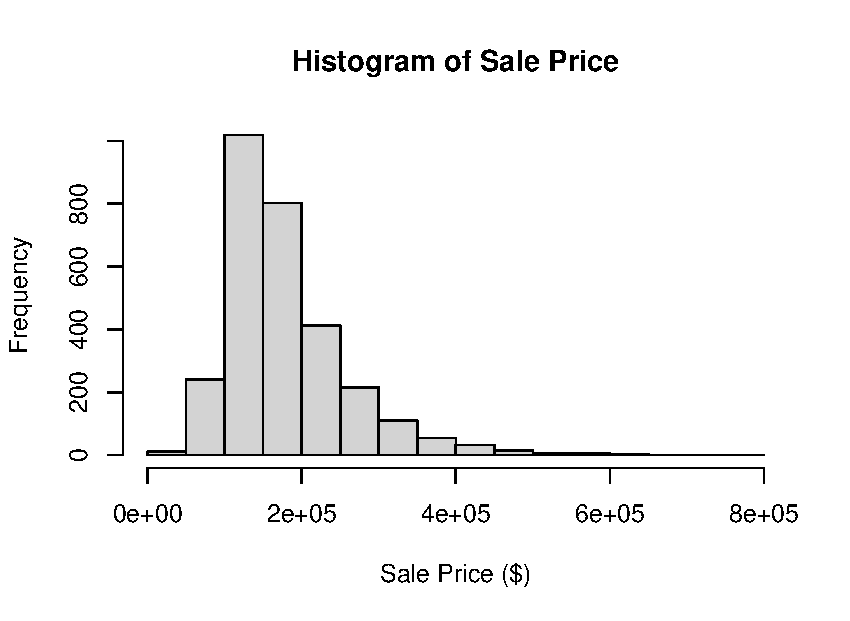
\includegraphics[width=0.6\textwidth]{fig/ex1.pdf}
\end{figure}
\emph{Explanation: 일변량 자료의 분포를 알아보는데 유용한 그래프는 히스토그램 hist()이다. SalePrice 변수에 대한 벡터를 데이터로부터 추출하여 히스토그램을 그려보면 right skewed된 분포를 확인할 수 있다. summary() 함수를 통해 5가지 통계량을 산출하였을 때 중간값이 평균보다 작은 것을 통해 히스토그램의 양상을 검증할 수 있다. } \\

(\textbf{Example 2}) 이 지역에서 발생한 전체 부동산 거래 가격의 평균값 $\mu$을 추정해보려고 한다. 지금처럼 모집단 전체를 알게 되는 경우는 매우 드물기 때문에 대부분의 경우에는 모집단
의 부분집합인 표본을 선택하여 모수를 추정하게 된다. \texttt{SalePrice}에서 50개의 랜덤 표본
을 선택해보자. 이 때, 모평균의 추정값은 무엇인가?
\begin{lstlisting}[style={r-style}]
saleprice.sample = sample(saleprice, 50, replace=F)
mean(saleprice); mean(saleprice.sample)
\end{lstlisting}
\begin{lstlisting}[style={out-style}]
[1] 180796.1
[1] 195056.3
\end{lstlisting}
\emph{Explanation: 모집단 saleprice에서 크기 50개의 표본을 추출하여 saleprice.sample에 저장하여 모집단 saleprice의 평균과 비교하면 서로 비슷한 값을 출력하는 것을 확인할 수 있다. 이를 통해 표본의 평균 (\$ 195,056) 으로 모평균 (\$ 180,796)을 추정할 수 있다.} \\

(\textbf{Example 3}) 예제 2의 과정을 5000번 반복하여 표본 평균의 표본 분포를 구해보자. 즉, 크기가 50인 랜덤 표본을 선택하여 표본평균을 구하는 과정을 5000번 반복하고 이 결과를
\texttt{sample\_mean50}이라는 이름의 벡터에 저장을 한다. \texttt{sample\_mean50}을 이용하여 히스토그램을 \texttt{sample\_mean50} 그려보자. 표본 평균의 분포는 어떠한가?
\begin{lstlisting}[style={r-style}]
sample_mean50 = c()
for (i in 1:5000) {
  saleprice.sample = sample(saleprice, 50, replace=F)
  sample_mean50[i] = mean(saleprice.sample)
}
hist(sample_mean50, xlim=c(140000, 230000),
     xlab="sample price ($)", main="Average sale price for sample size 50")
\end{lstlisting}
\begin{figure}[htb!]
    \centering
    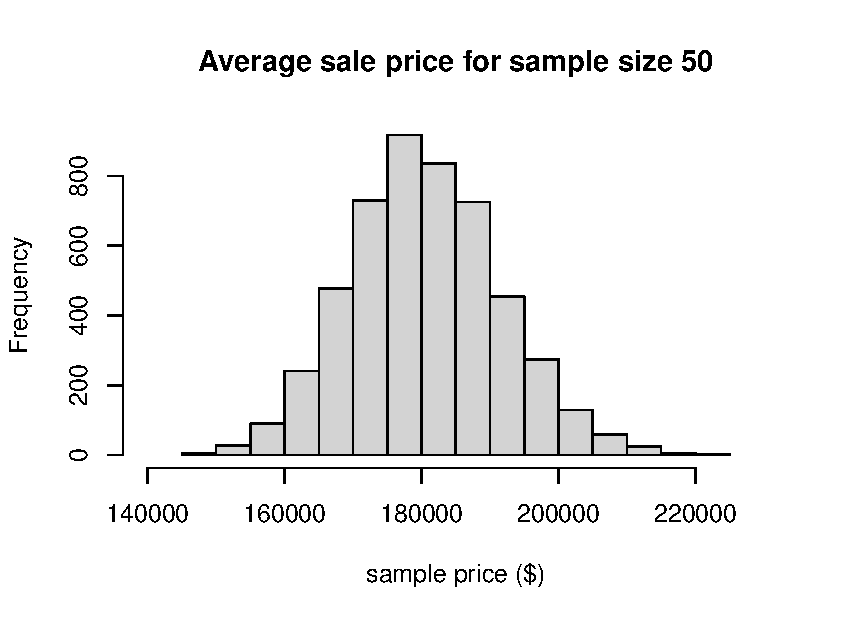
\includegraphics[width=0.6\textwidth]{fig/ex3.pdf}
\end{figure}
\emph{Explanation: \textbf{중심극한정리, CLT}, 평균이 $\mu$ 이고 분산이 $\sigma^2$인 임의의 무한 모집단에서 표본의 크기 $n$ 이 충분히 크면, 랜덤 표본의 표본평균은 근사적으로 정규분포 $N(\mu, \frac{\sigma^2}{n})$를 따른다. 표본의 크기 50인 sample price의 평균을 총 5,000번 구하고 히스토그램을 그리면 CLT에 의해 위의 도표처럼 근사적으로 정규분포를 따르는 것을 확인할 수 있다.} \\

(\textbf{Example 4}) 예제 3의 \texttt{sample\_mean50}의 평균과 분산을 계산해보자. \texttt{sample\_mean50}의 평균값은 모집단의 평균과 어떠한 관계가 있는가? \texttt{sample\_mean50}의 분산값은 모분산과 어떠한 관계가 있는가? 
\begin{lstlisting}[style={r-style}]
c(mean(sample_mean50), var(sample_mean50))
c(mean(saleprice), var(saleprice)/50)
\end{lstlisting}
\begin{lstlisting}[style={out-style}]
[1]    180569.7 120713851.8
[1]    180796.1 127637672.3
\end{lstlisting}
\emph{Explanation: CLT에 의해 랜덤 표본의 표본평균은 근사적으로 정규분포 $N(\mu, \frac{\sigma^2}{n})$를 따르므로, 표본평균의 분산과 모분산에 표본의 크기를 나누어준 결과를 서로 비교해주었다. 표본 평균과 모평균의 값은 서로 비슷하고 또한 표본평균의 분산값은 모분산과 n (표본의 크기)배 차이나는 것을 확인할 수 있다.}  \\

\newpage
(\textbf{Example 5}) 예제 3의 과정을 표본의 크기를 150으로 증가시켜 반복해보자. 이 결과는
\texttt{sample\_mean150}에 저장한다. 표본의 크기에 따른 표본 평균의 분포는 어떠한가?
\begin{lstlisting}[style={r-style}]
sample_mean150 = c()
for (i in 1:5000) {
  saleprice.sample = sample(saleprice, 150, replace=F)
  sample_mean150[i] = mean(saleprice.sample)
}
hist(sample_mean150, xlim=c(140000, 230000),
     xlab="sample price ($)", main="Average sale price for sample size 150")
\end{lstlisting}
\begin{figure}[htb!]
    \centering
    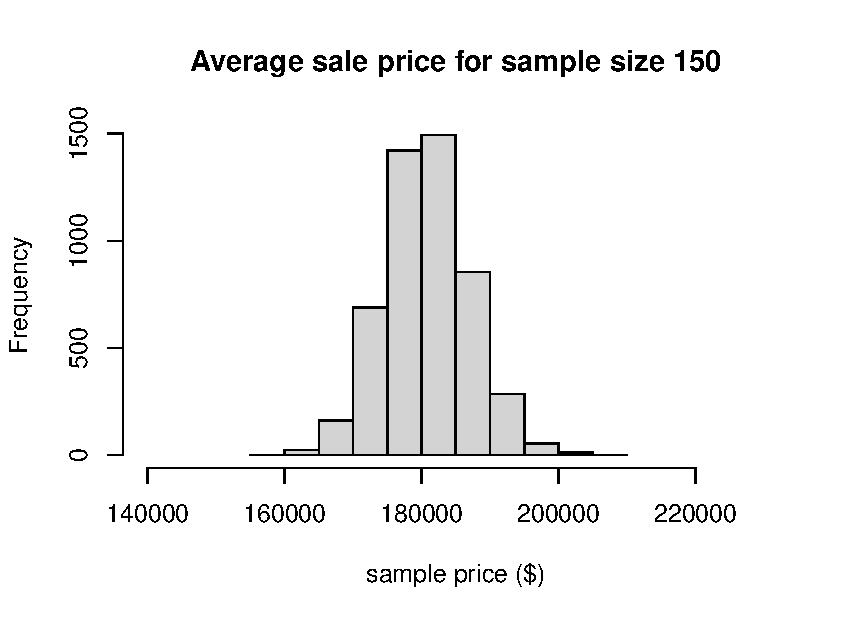
\includegraphics[width=0.6\textwidth]{fig/ex5.pdf}
\end{figure}
\emph{Explanation: 예제 3에서 했던 코드에서 표본의 크기 50을 150으로 변화시켜 히스토그램을 비교한다. 이때 표본 평균의 분포는 CLT에 의해 표본의 크기가 클 수록 근사적으로 정규분포를 따르게 된다. 표본의 크기 50에 비해 150의 히스토그램이 종 모양이 더 잘 형성된 것을 확인할 수 있다. } \\

\section*{Example 6}
강의노트 중 여러 가지 분포에서 카이제곱 분포 생성에서 자유도를 1, 5, 10, 30으로 변화시키면서 하나의 화면에 카이제곱 분포의 변화를 출력하도록 코딩하여라.
\begin{lstlisting}[style={r-style}]
f = c(1, 5, 10, 30)
par(mfrow=c(2,2))

for (i in 1:4) {
  xsquare.sum = c()
  for (j in 1:1000) {
    x = rnorm(f[i], mean=0, sd=1)
    xsquare.sum[j] = sum(x*x)
  }
  hist(xsquare.sum, probability=T, main=paste("chi-square ( f =", f[i], ")"))
  y = seq(0, max(xsquare.sum), 0.1)
  fy = dchisq(y, f[i])
  lines(y, fy)
}
dev.off()
\end{lstlisting}
\begin{figure}[htb!]
    \centering
    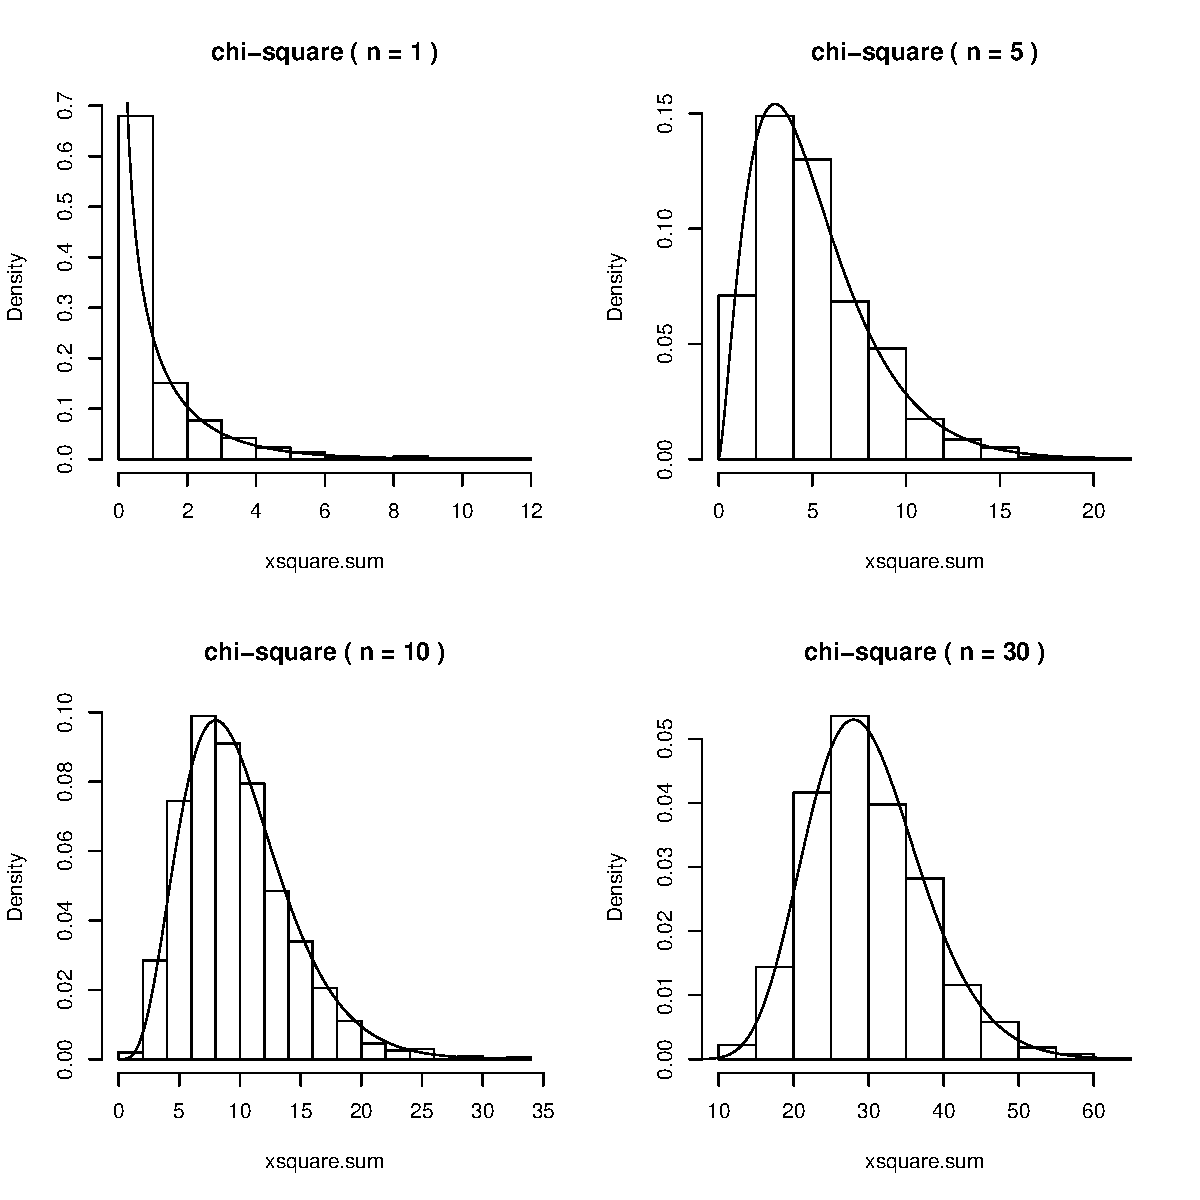
\includegraphics[width=0.8\textwidth]{fig/ex6.pdf}
\end{figure}
\emph{Explanation: 자유도 f에 벡터 1, 5, 10, 30을 저장하고 for 문을 활용해 2$\times$2 plot으로 표본의 갯수와 카이제곱의 확률밀도 함수를 출력하였다. 히스토그램의 도수를 확률로 출력하였고 실제 값을 lines로 출력한 결과와 상당히 유사한 분포로 출력되는 것을 확인하였다. } \\

\section*{Example 7}
어느 공장에서 생산하는 펜의 평균 사용 시간은 평균이 500 시간, 표준편차가 100 시간인 정규분포를 따른다고 한다. 이 공장 펜의 사용 시간이 800 시간 이하일 확률과 300 시간 이상일 확률을 구하여라. 
\begin{lstlisting}[style={r-style}]
mean = 500
sd = 100
pnorm(800, mean, sd)
pnorm(300, mean, sd, lower.tail=F)
\end{lstlisting}
\begin{lstlisting}[style={out-style}]
[1] 0.9986501
[1] 0.9772499
\end{lstlisting}
\emph{Explanation: 평균을 500 시간, 표준편차를 100 시간으로 변수에 대입하고 정규분포의 누적확률을 계산하는 pnorm()을 통해 800 시간 이하의 확률을 lower tail로 300 시간 이상의 확률을 upper tail로 계산하였다. } \\

\section*{Example 8}
정규분포 $N(100,36)$을 따르는 1000 개의 데이터를 생성하고, 생성된 데이터가 정규분포를 따르는지 \texttt{qqnorm()} 과 \texttt{qqline()}을 이용하여 확인하자. 
\begin{lstlisting}[style={r-style}]
par(mfrow=c(1,2))
data = rnorm(1000, mean=100, sd=36)
hist(data)
qqnorm(data)
qqline(data, col=2, lwd=3)
dev.off()
\end{lstlisting}
\begin{figure}[htb!]
    \centering
    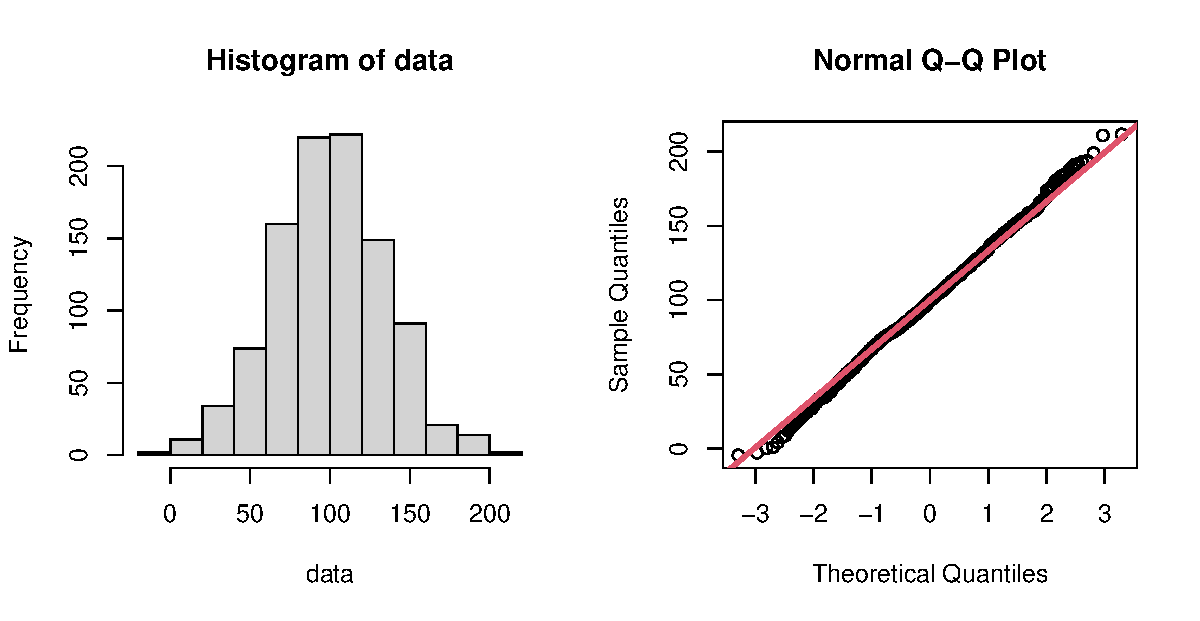
\includegraphics[width=0.8\textwidth]{fig/ex8.pdf}
\end{figure}
\emph{Explanation: 평균 100이고 분산이 36인 정규분포에서 1000개의 random sample을 rnorm() 함수를 이용해서 추출하였다. 이렇게 생성된 데이터로 히스토그램을 plot하고 정규분포 곡선과 비슷한 모양이 나오는 것을 확인하였다. 보다 정밀한 분석을 위해 정규분포 대조도 Q-Q plot을 qqnorm(), qqline()을 통해 도식화하였다. 직선에 모이는 것으로 보아 정규분포를 따른다고 말할 수 있다.} \\

\end{document}
